\documentclass[a4paper,11pt]{article}
\usepackage{dmasproject}
% if you need additional LaTeX packages, add them here
\usepackage[backend=biber]{biblatex}
\usepackage{amsthm}
\usepackage{enumitem}
\usepackage{mathtools}
\usepackage{cs73}
\usepackage{wrapfig}

\theoremstyle{definition}
\newtheorem{definition}{Definition}[section]

\theoremstyle{example}
\newtheorem*{example}{Example}

\theoremstyle{lemma}
\newtheorem{lemma}{Lemma}

\addbibresource{references.bib}

\newcommand{\lcalc}{\lambda\text{-calculus}}
\newcommand{\bred}{\beta\text{-reduction}}
\newcommand{\lamterm}[2]{\lambda #1. #2}
\newcommand{\subs}[3]{#1[#2\coloneqq#3]}
\newcommand{\redto}{\longrightarrow}
\newcommand{\ssbr}{\rightarrow_{\beta}}
\newcommand{\msbr}{\twoheadrightarrow_{\beta}}
\newcommand{\pbr}{\rightrightarrows_{\beta}}
\newcommand{\tssbr}{\text{single-step $\beta$-reduction}}
\newcommand{\tmsbr}{\text{multi-step $\beta$-reduction}}

\title{Lambda Calculus and The Church-Rosser Theorem}
\author{Ke Wu}

%TODO: find all \equiv for substitution and change them to =

\begin{document}

\maketitle

\tableofcontents

\newpage

\section{Introduction}

\textit{``Entscheidungsproblem"}, or the ``Decision Problem", proposed by David Hilbert and Wilhelm Ackermann in 1928, asks for a general algorithm that, when given a set of logic rules and a logical statement, decided whether the given statement is valid (i.e. provable using the given rules or axioms). Formally introduced by Alonzo Church in the 1930s, Lambda Calculus ($\lcalc$) is a formal system invented to address this problem, or as it turned out, to demonstrate that this problem cannot be addressed. Along with the Turing machine model (named after its inventor, Alan Turing), they served as the theoretical foundation to a negative answer to the Decision Problem\cite{Barendregt2000}.

The Turing machine model continued to thrive as a model of computation, eventually leading to the invention of modern computers and the birth of Computer Science as a new discipline. However, $\lcalc$ seemed to remain only a formalism. Fortunately, the potential of $\lcalc$ was rediscovered around 1960s, when scientists began to notice the connection between $\lcalc$ and various areas of study, e.g. functional programming languages, and semantics of natural language. Since then, $\lcalc$ has been serving as an important theoretical foundation to many functional languages and related research\cite{sep-lambda-calculus}.

In this paper, I will provide a general introduction to the pure $\lcalc$ and a proof to the Church-Rosser Theorem, one of the key theorems related to $\lcalc$.

\section{Syntax and Semantics of $\lcalc$}

Consider a simple function, $f(x) = x^2 + 2x + 1$. We can easily ask the question: ``What is the value of this polynomial when $x = 1$?" To find out the answer, we simply substitute the value $1$ for $x$ in the polynomial, and compute the result (in this case, we have $f(1) = 1^2 + 2\cdot 1 + 1 = 4$). The core of $\lcalc$ is to capture this idea of substitution, or to put it more formally, the idea of ``function application". In $\lcalc$, we can express the polynomial as a $\lambda$-term, $\lamterm{x}{(x^2 + 2x + 1)}$. Intuitively, the notation ``$\lambda$x" in the expression has a very similar function to $f(x)$ in the polynomial: it tells us what the variable is in the body. I will discuss this concept in more detail later. 

We can \textit{apply} this expression to an \textit{argument} to get its value. We write `$Fa$" to denote the application of $F$ on the argument $a$. As with the previous example, the argument is $1$, so we have:
$$(\lamterm{x}{(x^2 + 2x + 1)})1\redto 1^2 + 2 \cdot 1 + 1 = 4$$
In fact, this example doesn't quite demonstrate the actual $\lcalc$, since ``numbers" as we know them do not actually exist in $\lcalc$; instead, they are encoded using functions. A more realistic example of $\lcalc$ would be the following:
$$(\lamterm{x}{xx})y\redto yy$$
As ridiculous as this example might look, we can see that the idea of \textit{substitution} is really at the heart of $\lcalc$; even with bare symbols, the rule of substitution still holds as we imagine it will. This illustrates the central axiom of $\lcalc$: $\bred$. Intuitively, this axiom simply dictates that given a $\lambda$-term $(\lamterm{x}{M})$, $\bred$ will replace every instance of $x$ (the bound variable) in the expression $M$ with the argument $N$. I will discuss this axiom in more detail later.

\subsection{Syntax}
In this section, I will formally introduce $\lcalc$.

\theoremstyle{definition}
\begin{definition}{}
The alphabet of $\lcalc$ is the set $\{``\lambda", ``(", ``)", ``."\}\cup V$,
where $V$ is an infinite set of \textit{\textbf{variables}}: $\{v_0, v_1, \dots\}$. \textit{\textbf{$\lambda$-terms}} are words over the alphabet, defined inductively as follows:
\begin{enumerate}[topsep=1pt,itemsep=-1ex,partopsep=1ex,parsep=1ex]
    \item $x$ is a $\lambda$-term for any variable $x \in V$.
    \item If $M$ and $N$ are $\lambda$-terms, then $(MN)$ is a $\lambda$-term. \textbf{(Application)}
    \item If $M$ is a $\lambda$-term, and $x \in V$, then $(\lamterm{x}{M})$ is a $\lambda$-term. \textbf{(Abstraction)}
\end{enumerate}
\end{definition}
Using our previous example, the term $(\lamterm{x}{xx})$ is a $\lambda$-term constructed using rule (3), while the term $((\lamterm{x}{xx})y)$ is constructed with rule (2).

To avoid any notational ambiguity, I will adopt the following conventions for the rest of the paper:
\begin{enumerate}[topsep=1pt,itemsep=-1ex,partopsep=1ex,parsep=1ex]
    \item Lowercase letters represent arbitrary variables, and uppercase letters represent arbitrary $\lambda$-terms.
    \item We can omit parentheses in applications by \textit{\textbf{left-associativity}}, meaning that when we have more than two terms strung together, e.g. $M_1M_2M_3\dots M_n$, it's interpreted as $(\dots((M_1M_2)M_3)\dots M_n)$.
    \item Abstraction, on the other hand, is \textit{\textbf{right-associative}}, meaning $\lamterm{x}{\lamterm{y}{\lamterm{z}{xyyz}}} \equiv \lamterm{x}{(\lamterm{y}{(\lamterm{z}{xyyz})})}$. For functions with multiple arguments, i.e. $\lamterm{x_1}{(\lamterm{x_2}{\dots(\lamterm{x_n}{M})})}$, we can use the shorthand notation $\lamterm{x_1\dots x_n}{M}$.
\end{enumerate}

\subsection{Free vs. Bound variables}
As promised earlier, I will unveil the mystery of $\lambda x$ now. In an abstraction term, $\lamterm{x}{M}$, the use of the $\lambda$ symbol is to \textit{\textbf{bind}} the variable $x$ in the term $M$. It is very similar to the function of universal and existential quantifiers, $\forall$ and $\exists$, in first-order logic. Formally, we can define the concepts of free and bound variables as follows:
\theoremstyle{definition}
\begin{definition}{}
\textit{\textbf{FV(M)}} is the set of free variables in $M$, defined by these inductive rules:
\begin{enumerate}[topsep=1pt,itemsep=-1ex,partopsep=1ex,parsep=1ex]
    \item $FV(x) = \{x\}$
    \item $FV(MN) = FV(M) \cup FV(N)$
    \item $FV(\lamterm{x}{M}) = FV(M) - \{x\}$
\end{enumerate}
A variable is \textit{\textbf{bound}} in $M$ if it is not free. Intuitively, if a variable $x$ appears under the scope of a $\lambda x$, then it is bound.
\end{definition}

\begin{example}{}
Consider the expression $M = \lamterm{xy}{xyz}$. What is $FV(M)$?
\end{example}

\begin{proof}
First, let's rewrite $M$ in the form of explicit abstraction: $M \equiv \lamterm{x}{(\lamterm{y}{xyz})}$. By rule (1), we have $FV(x) = \{x\}$, $FV(y) = \{y\}$, $FV(z) = \{z\}$. By rule (2), we have $FV(xyz) = FV(x) \cup FV(y) \cup FV(z) = \{x, y, z\}$. By rule (3), we have $FV(\lamterm{y}{xyz}) = FV(xyz) - \{y\} = \{x, z\}$. Similarly, $FV(\lamterm{x}{(\lamterm{y}{xyz})}) = FV(\lamterm{y}{xyz}) - \{x\} = \{z\}$. Therefore, we have $FV(M) = FV(\lamterm{x}{(\lamterm{y}{xyz})}) = \{z\}$. It follows naturally that the bound variables in $M$ are $\{x, y\}$.
\end{proof}

\subsection{Substitution}
Before introducing the formal theory of $\lcalc$, we need to understand how substitution works for $\lambda$-terms.

\begin{definition}
We write $\subs{M}{x}{N}$ to represent the function substituting all \textit{free} occurrences of $x$ in $M$ with the term $N$. The precise definition of substitution is defined inductively as follows:
\begin{enumerate}[topsep=1pt,itemsep=-1ex,partopsep=1ex,parsep=1ex]
    \item $\subs{x}{x}{M} = M$
    \item $\subs{y}{x}{M} = y$ $(y \neq x)$
    \item $\subs{(AB)}{x}{M} = \subs{A}{x}{M}\subs{B}{x}{M}$
    \item $\subs{(\lamterm{x}{A})}{x}{M} = \lamterm{x}{A}$
    \item $\subs{(\lamterm{y}{A})}{x}{M} = \lamterm{y}{(\subs{A}{x}{M})}$ $(y \neq x)$
\end{enumerate}
\end{definition}
Rule (1) and (2) are the base cases for substitution, where the term we are dealing with is a single variable. If the variable matches the one we are currently substituting, then we replace the variable with the corresponding expression; if the variable does not match, we do not perform any substitution. Rule (3) dictates that substitution distributes over application. Rule (4) reiterates the fact that we are only substituting all \textit{free} occurrences; if the variable we are substituting is bound by a $\lambda$ in the term, then we do not perform any substitution. Rule (5) states that if the bound variable is different, then we can perform substitution on the body of the abstraction term.

\begin{example}
Consider the substitution, $\subs{(x(\lamterm{x}{y}))}{x}{z}$. What is the result of this substitution?
\end{example}
\begin{proof}
In this case, we can first apply rule (3), setting $A = x$, $B = \lamterm{x}{y}$, $M = z$. By rule (3), we can then consider $\subs{A}{x}{M}\subs{B}{x}{M}$, i.e. the term becomes $\subs{x}{x}{z}\subs{(\lamterm{x}{y})}{x}{z}$. Rule (1) applies directly to $\subs{x}{x}{z}$, from which we get $\subs{x}{x}{z} = z$. Since $z \neq x$, rule (4) applies to $\subs{(\lamterm{x}{y})}{x}{z}$, from which we get $\subs{(\lamterm{x}{y})}{x}{z} = \lamterm{x}{y}$. We can combine these two results, and conclude that the final result of the substitution is $z(\lamterm{x}{y})$.
\end{proof}

Now, consider these two $\lambda$-terms: $\lamterm{x}{x}$ and $\lamterm{y}{y}$. The only difference between these two terms is the name of the variable, and very much like mathematical functions, changing the name of the variable should not change the functions themselves. For example, the function $f(x) = 2x + 1$ is exactly the same as $f(y) = 2y + 1$. To capture this natural equivalence through renaming in $\lcalc$, we define the concept of $\alpha$-conversion as follows:

\begin{definition}
\textbf{($\alpha$-conversion)} For any $\lambda-$term $M$, we can perform \textit{\textbf{$\alpha$-conversion}} to get an equivalent $\lambda-$term $N$ by replacing $v$ with $v'$ for all abstraction term $\lamterm{v}{A}$ in $M$, given that $v'$ does not occur in $A$. We say that terms $M$ and $N$ are \textit{\textbf{$\alpha$-convertible}} if we can perform a series of $\alpha$-conversion to get from $M$ to $N$. 
\end{definition}

Now we have everything we need to finally introduce $\beta$-reduction, the central axiom of $\lcalc$:
\begin{definition}\textbf{($\beta$-reduction)}
For all $\lambda$-terms $M, N$, 
$$(\lamterm{x}{M})N \redto \subs{M}{x}{N}$$
provided that no free variables in $N$ becomes bound after its substitution into $M$.
\end{definition}

Essentially, the extra condition on $\beta$-reduction is to make sure that free variables remain free. The importance of this condition can be best illustrated with some examples.

\begin{example}
Consider the $\lambda$-term, $(\lamterm{x}{(\lamterm{y}{x})})y$. What should the substitution result be?
\end{example}

If we perform the substitution as it is right now, we will have $(\lamterm{x}{(\lamterm{y}{x})})y \redto \subs{\lamterm{y}{x}}{x}{y}$, and by substitution rule (5) and (1), we have $\subs{\lamterm{y}{x}}{x}{y} = \lamterm{y}{y}$. However, does not satisfy our condition for using $\beta$-reduction: we require that no free variables in $N$ becomes bound after the substitution. The variable $\lambda$-term $y$ corresponds to $N$ in this case, and we can see that it changes from free to bound after we perform the substitution. The intuition behind why we don't want this to happen is that, although they have the same name, $y$, the inner one bound by $\lambda$ is really referring to a \textit{different} variable than the outermost $y$.

This is where $\alpha$-conversion comes in rescue. Since it should not matter what name we give to the binding variable, we can simply rename the inner binding expression from $\lamterm{y}{x}$ to $\lamterm{z}{x}$, i.e. $(\lamterm{x}{(\lamterm{y}{x})})y \equiv (\lamterm{x}{(\lamterm{z}{x})})y$. Note that since the bound variable did not appear in the body anywhere in the first place, we do not have to perform any further name-changing in the body either. After $\alpha$-conversion, we can now safely use $\beta$-reduction to get the result we would expect: $(\lamterm{x}{(\lamterm{z}{x})})y \redto \subs{\lamterm{z}{x}}{x}{y} = \lamterm{z}{y}$.
\subsection{Reduction}

However, $\beta$-reduction alone is still not quite enough for us to exploit the full potential of $\lcalc$. Consider the following example:

\begin{example}
Consider the $\lambda$-term, $\lamterm{x}{((\lamterm{y}{y})z)}$. Is it true that $\lamterm{x}{((\lamterm{y}{y})z)} \redto \lamterm{x}{z}$? Can you prove it?
\end{example}
Intuitively, we know this statement should be true, since the subterm $(\lamterm{y}{y})z = z$ by our laws of substitution. However, the $\beta$-reduction rule as it is now only allows us to perform substitution when we have an application term at the outermost level, i.e. when we have a $\lambda$-term $M$ such that $M = (\lamterm{x}{M'})N$ for some other $\lambda$-term $M', N$. Since our $\lambda$-term is an abstraction term, it does not fit the form required by the rule. This suggests that we are still missing some essential rules.

To solve the problem that arose in the last section, we now define the binary relations $\ssbr$ \textbf{(\tssbr)} and $\msbr$ \textbf{(multi-step $\beta$-reduction)} on $\lambda$-terms. Together they will be the complete definition for $\beta$-reduction.
\begin{definition}
The binary relations $\ssbr$ and $\msbr$ are defined inductively as follows: 
\begin{enumerate}[topsep=2pt,itemsep=-0.5ex,partopsep=1ex,parsep=1ex]
    \item \begin{enumerate}[topsep=2pt,itemsep=-0.5ex,partopsep=1ex,parsep=1ex]
        \item $(\lamterm{x}{M})N \ssbr \subs{M}{x}{N}$
        \item $M \ssbr N \implies ZM \ssbr ZN$ $\quad$
        \item $M \ssbr N \implies MZ \ssbr NZ$
        \item $M \ssbr N \implies \lamterm{x}{M} \ssbr \lamterm{x}{N}$
    \end{enumerate}
    \item \begin{enumerate}[topsep=2pt,itemsep=-0.5ex,partopsep=1ex,parsep=1ex]
        \item $M \msbr M$
        \item $M \ssbr N \implies M \msbr N$
        \item $M \msbr N, N \msbr L \implies M \msbr L$
    \end{enumerate}
\end{enumerate}
\end{definition}
As the name suggests, $\tssbr$ represents one single step of $\beta$-reduction, i.e. performing substitution once on the given $\lambda$-term. Intuitively, $\tmsbr$ represents a \textit{sequence} of substitutions on the given term.

Now with this more robust definition for $\beta$-reduction, we can come back to the example and see how it can be proven in the new system.

\begin{example}
Show that $\lamterm{x}{((\lamterm{y}{y})z)} \ssbr \lamterm{x}{z}$.
\end{example}
\begin{proof}
By rule 1(a), we know that $(\lamterm{y}{y})z \ssbr \subs{y}{z}{y} = z$. Then, by rule 1(d), let $M = (\lamterm{y}{y})z$, $N = z$, we have $\lamterm{x}{M} \ssbr \lamterm{x}{N}$, i.e. $\lamterm{x}{((\lamterm{y}{y})z)} \ssbr \lamterm{x}{z}$.
\end{proof}

\begin{definition}\ 
\begin{enumerate}[topsep=2pt,itemsep=-0.5ex,partopsep=1ex,parsep=1ex]
    \item A \textbf{\textit{$\beta$-redex}} is a term of the form $(\lamterm{x}{M})N$. We call $\subs{M}{x}{N}$ its \textit{contractum}. 
    \item $M$ \textit{\textbf{is a $\beta$-normal form ($\beta$-nf)}} if it doesn't contain any $\beta$-redexes as its subterms.
    \item $M$ \textit{\textbf{has a $\beta$-normal form}} if there exists a $\beta$-normal term $N$ and that $M \msbr N$.
\end{enumerate}
For example, the term $(\lamterm{x}{(\lamterm{y}{y})})z$ is a $\beta$-redex, and its contractum is $\subs{\lamterm{y}{y}}{x}{z}$. Since $(\lamterm{x}{(\lamterm{y}{y})})z$ is a $\beta$-redex, we know that it is not a $\beta$-normal form. However, it does have the $\beta$-normal form $\lamterm{y}{y}$ after we perform the substitution.

\end{definition}

\section{Induction on Proof Tree}

\begin{wrapfigure}{r}{0.3\textwidth}
  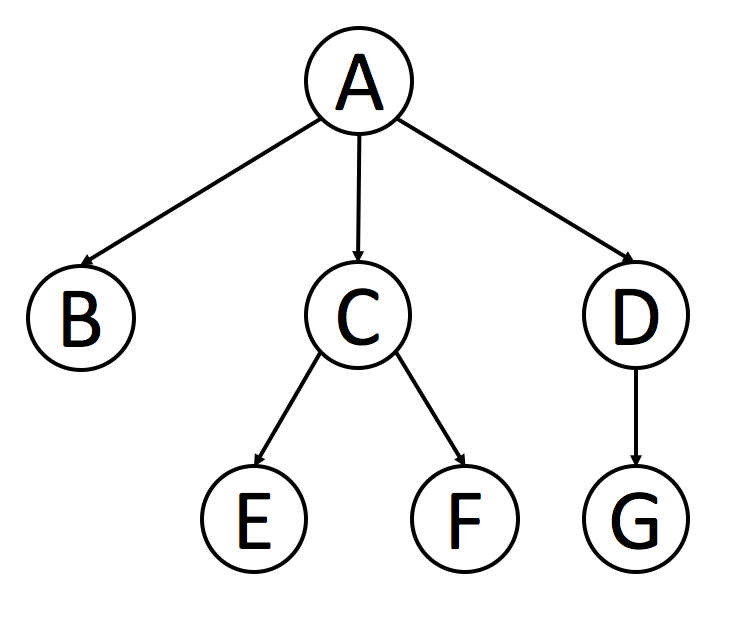
\includegraphics[scale=0.35]{tree_example.png}
  \caption{Example Tree}
\end{wrapfigure}

Before getting to the main theorem of this paper, there is one important detour we need to make. In this section, I will introduce the perspective of seeing proofs as mathematical structures, and performing induction on them. This idea will be key to proving the Church-Rosser Theorem.

\subsection{The World of Trees}
Trees. Alveoli of the Earth, home to squirrels and birds, origin of this piece of paper. There are many things we can say about trees, but above all, we don't have enough of them. Unfortunately, those trees (and related environmental concerns) are not the focus of this section. Recall another definition of tree you might have encountered in graph theory:
\begin{definition}
A \textbf{\textit{tree}} is a connected acyclic undirected graph. A \textbf{\textit{rooted tree}} is a tree where a special node is singled out as the ``root''. In a rooted tree, the \textbf{\textit{parent}} of a node $x$ is the node $y$ connected to $x$ on the path to the root. We also define $x$ as the \textbf{\textit{child}} of $y$. If a node has no child nodes, we call it a \textbf{\textit{leaf node}}.
\end{definition}

\begin{example}
In figure 1, if $A$ is the root node, which nodes are the leaf nodes? Which node(s) have $C$ as their parent? Which node is the child node of $D$?
\end{example}
The leaf nodes are $B, E, F$, and $G$. And $E, F$ have $C$ as their parent node. Finally, $G$ is the child node of $D$.

\subsection{Induction on Trees}
There are a few other key terms about trees that we need to introduce:
\begin{definition}
The \textbf{\textit{height}} of a node $u$ is the length of the longest path from $u$ to any leaf. A leaf node has height $0$. The height of a tree is defined as the height of its root node.
\end{definition}
\begin{example}
What is the height of the node $C$ in figure 1? What about the height of the tree?
\end{example}
Since the longest path length from $C$ to any leaf node ($E$ or $F$) is $1$, we know $C$ has height $1$. Since $A$ is the root node, the height of the tree is $2$.

Since the root node always has the biggest height, and that all child nodes will have a lesser height than their parent node, we can in fact perform mathematical induction on the height of the tree. I will demonstrate by the following example.

\begin{example}
Let $T$ be a tree in which every node can have at most $2$ child nodes, and the height of $T$ is $h$. What is the maximum number of nodes (denoted as $n$) we can have in the tree?
\end{example}
\noindent\textbf{Claim: }There can be at most $2^{h+1} - 1$ nodes.
\begin{proof}
I will prove the claim by induction on the height of the tree.

\textbf{Base case: }$h = 0$. This suggests that the root node is a leaf node. Therefore, we know the root node is the only node in the tree, thus $n = 1$. Since $2^{0+1} - 1 = 1$, we can conclude $n \leq 2^{h+1} - 1$. Thus the base case holds.

\textbf{Induction hypothesis: }For $h < k$, we have $n \leq 2^{h+1} - 1$.

\textbf{Inductive Step: }$h = k$. In this case, we want to show that this tree has at most $2^{k+1} - 1$ nodes. We know that the root node has height $k$, and its child node has height $k-1$. By the induction hypothesis, we know that each child node of the root can have at most $2^{k-1+1}-1$ nodes in their corresponding subtree. Therefore, this tree have at most $2(2^{k}-1) + 1 = 2^{k+1} - 1$ nodes. Thus we have established the claim.

\end{proof}

\subsection{Proof as Tree}
Traditionally, when we think about proofs using inference rules, we tend to think of them as linear or sequential. However, we can also represent proofs as a tree structure.

\begin{definition}
A \textit{\textbf{Proof Tree}} is a finite tree where each node is a rule, and the subtree rules have conclusions which exactly match the parent's premises. All leaves of a proof tree must be axioms. A tree with a non-axiom leaf is not a proof.
\end{definition}

A conventional way to visualize proof trees is using this form:
\begin{mathpar}
    \ir[]{A \quad B}{C}
\end{mathpar}
where $A, B$ are the \textit{\textbf{premises}} and $C$ is the \textit{\textbf{conclusion}}. This is equivalent to the statement: ``$A$ and $B \implies C$". Note that in this representation, premises are separated by white spaces. 

Unlike the tree in the previous example, proof trees are oriented like an actual ``tree", i.e.: the root node is at the bottom, containing the statement we want to prove as its conclusion. The subtrees are the child nodes positioned above the root node, and they represent subproofs that are needed to reach the final conclusion.

Now that we have defined proofs as trees, we can proceed to establish proof by induction on the height of proof trees in the next section.

\subsection{Compatibility of $\beta$-reduction}
One key property of $\tssbr$ and $\tmsbr$ is \textbf{\textit{compatibility}}; we will define compatibility formally in this section, and prove that both relations satisfy the criteria. We will make use of this property in our proof of the central theorem.

\begin{definition}
A binary relation $R$ on $\lambda$-terms is \textit{\textbf{compatible}} if it satisfies the following rules for any $\lambda$-terms $M, R, N$:
\begin{enumerate}[topsep=2pt,itemsep=-0.5ex,partopsep=1ex,parsep=1ex]
    \item $M\ R\ N \implies (ZM)\ R\ (ZN)$
    \item $M\ R\ N \implies (MZ)\ R\ (NZ)$
    \item $M\ R\ N \implies \lamterm{x}{M}\ R\ \lamterm{x}{N}$
\end{enumerate}
\end{definition}

A good example of a compatible relation is \textit{\textbf{equality}} of $\lambda$-terms; if two terms $M$ and $M'$ are equal, then no matter how many abstractions and applications we perform on them (at the same time), the resulting terms will still be equal. 

\begin{lemma}
$\ssbr$ and $\msbr$ are compatible on $\lambda$-terms.
\end{lemma}
\begin{proof}(Compatibility of $\ssbr$)
First, we can easily show that $\ssbr$ is compatible by its definition. Rule 1(b), 1(c), and 1(d) of Definition 2.6 correspond to the three conditions of compatibility directly, so we can safely conclude that $\ssbr$ is a compatible relation.
\end{proof}
\begin{proof}(Compatibility of $\msbr$)
This proof is less straightforward. Essentially, we'd like to show that the following properties hold for $\msbr$:
\begin{enumerate}[topsep=2pt,itemsep=-0.5ex,partopsep=1ex,parsep=1ex]
    \item $M \msbr N \implies ZM \msbr ZN$
    \item $M \msbr N \implies MZ \msbr NZ$
    \item $M \msbr N \implies \lamterm{x}{M} \msbr \lamterm{x}{N}$
\end{enumerate}
Let's focus on the first property. Since it is a rule of inference, we can assume the premise, $M \msbr N$, is true. Therefore, there must exists some proof tree, $T$, for $M \msbr N$. We will proceed to prove this rule by \textit{strong induction on the height of $T$}.

\textbf{Base case: }The height of $T$ is $0$. As we discussed before, this indicates that $T$ is an axiom. Since the only axiom we have for $\msbr$ is $M \msbr M$ (the identity rule), we know this is the only possible candidate for $T$. This suggests that $M = N$, and by compatibility of equality, we know that $ZM = ZN$. Then we can apply the identity rule again, and get $ZM \msbr ZN$. Thus we have shown the base case holds.

\textbf{Induction Hypothesis: }For proof tree with height less than $h$, $M \msbr N \implies ZM \msbr ZN$.

\textbf{Inductive Step: }We want to show that when we have a proof tree with height $h$ for $M \msbr N$, we can prove $ZM \msbr ZN$. Since we have more than one rules that will allow us to prove the premise $M \msbr N$, we will perform a case analysis on all the possible ways to generate the proof for $M \msbr N$ (the rules are listed in Def 2.6).
\begin{enumerate}[topsep=2pt,itemsep=-0.5ex,partopsep=1ex,parsep=1ex]
    \item $M \ssbr N \implies M \msbr N$: If this rule is used to generate the proof for $M \msbr N$, we know that there must exist some proof for the premise, $M \ssbr N$. Since we've shown $\ssbr$ is a compatible relation, we know that $M \ssbr N \implies ZM \ssbr ZN$. We can then apply rule 2(b) again to get $ZM \msbr ZN$. 
    \item $M \msbr L, L \msbr N \implies M \msbr N$: If this rule is used to generate the proof for $M \msbr N$, we know that there must exist some proofs for the premises, $M \msbr L$ and $L \msbr N$. Since both proofs need to be subtrees of our current tree, we know they must have height less than $h$. By the induction hypothesis, we know that $ZM \msbr ZL$ and $ZL \msbr ZN$. Then, we can apply rule 2(c) to get $ZM \msbr ZN$.
\end{enumerate}
Since these are the only rules we could have used to generate a proof for $M \msbr N$, and that we've shown in both cases, we can then produce a proof for $ZM \msbr ZN$, we can safely conclude that $M \msbr N \implies ZM \msbr ZN$.

The proofs of property 2 and 3 are very similar, so I will omit it here for brevity.
\end{proof}


% \section{$\lcalc$ in action}

% \subsection{Combinators}
% \subsection{Church numerals}
% (May only keep one of them if there's not enough room)

% \section{Reduction}

% In the previous section, we walked through a general definition of reduction and the intuition behind it. However, to approach the Church-Rosser Theorem, we need to understand reduction more formally first.

% \begin{definition}
% A binary relation $R$ on $\lambda$-terms is \textit{compatible} if it satisfies the following rules:
% \begin{enumerate}[topsep=2pt,itemsep=-0.5ex,partopsep=1ex,parsep=1ex]
%     \item $M\ R\ N \implies (ZM)\ R\ (ZN)$
%     \item $M\ R\ N \implies (MZ)\ R\ (NZ)$
%     \item $M\ R\ N \implies \lamterm{x}{M}\ R\ \lamterm{x}{N}$
% \end{enumerate}
% \end{definition}
% These rules might look familiar, because they are part of the inference rules we have for equality of $\lambda$-terms. This shows us that equality on $\lambda$-terms is a compatible relation.

% Now, we are going to introduce two more binary relations on $\lambda$-terms.

% \begin{definition}
% The binary relations $\ssbr$ \textbf{(\tssbr)} and $\msbr$ \textbf{(multi-step $\beta$-reduction)} on $\lambda$-terms are defined inductively as follows: 
% \begin{enumerate}[topsep=2pt,itemsep=-0.5ex,partopsep=1ex,parsep=1ex]
%     \item \begin{enumerate}[topsep=2pt,itemsep=-0.5ex,partopsep=1ex,parsep=1ex]
%         \item $(\lamterm{x}{M})N \ssbr \subs{M}{x}{N}$
%         \item $M \ssbr N \implies ZM \ssbr ZN$
%         \item $M \ssbr N \implies MZ \ssbr NZ$
%         \item $M \ssbr N \implies \lamterm{x}{M} \ssbr \lamterm{x}{N}$
%     \end{enumerate}
%     \item \begin{enumerate}[topsep=2pt,itemsep=-0.5ex,partopsep=1ex,parsep=1ex]
%         \item $M \msbr M$
%         \item $M \ssbr N \implies M \msbr N$
%         \item $M \msbr N, N \msbr L \implies M \msbr L$
%     \end{enumerate}
% \end{enumerate}
% \end{definition}


% By definition, $\ssbr$ is a compatible relation. Though not explicitly defined as such, we can show that $\msbr$ is also compatible.

% \begin{lemma}
% $\msbr$ is a compatible relation.
% \end{lemma}

% \begin{proof}
% To prove that $\msbr$ is a compatible relation, we need to show that it satisfies the three rules listed in Definition 4.1.
% \begin{enumerate}[topsep=2pt,itemsep=-0.5ex,partopsep=1ex,parsep=1ex]
%     \item $M \msbr N \implies (ZM) \msbr (ZN)$: 
% \end{enumerate}
% \end{proof}

\section{The Church-Rosser Theorem}

So far we've been dealing with rather simple $\lambda$ expressions; none of the examples made use of the $\tmsbr$ definition because they never required more than one step of $\beta$-reduction. One natural question to ask is: How does our system behave when given a more complicated expression? 

\begin{example}
Consider the expression $(\lamterm{x}{(\lamterm{y}{y})x})z$. What does it reduce to?
\end{example}

Ok. Houston, we have a problem. Since there are two $\beta$-redexes in this expression, we have more than one way to reduce it: we can either reduce the inner application first (i.e. $\subs{y}{y}{x}$), or the outer application (i.e. $\subs{(\lamterm{y}{y})x}{x}{z}$). Our system does not include any rule that dictates the order of reduction, so either option is valid. However, you might also notice that no matter which expression we choose to reduce first, once we perform one more reduction, we will end up with the same expression, namely $z$. It looks like no matter what order of reduction we choose, we will eventually get the same result. 

``But is this always true? Does the order of reduction not matter for all expressions?" 

I'm glad you asked! It turns out that in Untyped $\lcalc$, the order of reduction really does not matter in that all orders can lead to the same conclusion eventually. This is the core of the Church-Rosser Theorem. I will state the theorem formally next, and present Takahashi's proof\cite{TAKAHASHI1989113} of this theorem, which is based on the idea of parallel reduction.

\theoremstyle{plain}
\newtheorem*{crt}{Church-Rosser Theorem}
\begin{crt}
If $M \msbr N_1$, $M \msbr N_2$, then there exists a term $N_3$ such that $N_1 \msbr N_3$ and $N_2 \msbr N_3$.
\end{crt}

The Church-Rosser Theorem has many important implications, but the two listed below are the most widely recognized/researched.
\vspace{-2mm}
\begin{enumerate}[noitemsep]
  \item It establishes the potential for \textbf{concurrency} in reduction. This is especially useful in Computer Science; parallelization can greatly improve performance of program. 
  \item It allows different \textbf{reduction strategies} for different expressions. Sometimes one strategy might cause the program to get stuck in an infinite loop; the flexibility offered by the Church-Rosser Theorem allows programs to potentially avoid infinite loops.
\end{enumerate}
\vspace{-2mm}

The proof of this theorem can be broken down into roughly three parts: first, we want to introduce (yet another!) binary relation on $\lambda$-terms, \textit{\textbf{parallel reduction}}, and establish certain properties that parallel reduction has with respect to $\tssbr$ and $\tmsbr$. Then, we want to discuss how we will relate a key property of parallel reduction to the Church-Rosser Theorem. Finally, we will demonstrate the proof of that key property, and thus proving the Church-Rosser Theorem.

\subsection{Parallel $\beta$-Reduction}
\begin{definition}
We inductively define $\pbr$, the parallel $\beta$-reduction, as follows:
\begin{enumerate}[topsep=2pt,itemsep=-0.5ex,partopsep=1ex,parsep=1ex]
    \item $x \pbr x$
    \item $M \pbr M' \implies \lamterm{x}{M} \pbr \lamterm{x}{M'}$
    \item $M \pbr M', N \pbr N' \implies MN \pbr M'N'$
    \item $M \pbr M', N \pbr N' \implies (\lamterm{x}{M})N \pbr \subs{M'}{x}{N'}$
\end{enumerate}
The first three rules dictate that in this system, we have $M \pbr M$ holds for all $\lambda$-term $M$. The fourth rule is more subtle; when used in tandem with the third rule, it essentially allows us to contract some $\beta$-redexes (possibly overlapping) in $M$ simultaneously to obtain $M'$.
\end{definition}
Now, we will relate $\pbr$ with $\ssbr$ and $\msbr$ with the following lemmas:
\begin{lemma}
$M \ssbr M' \implies M \pbr M'$.
\end{lemma}
\begin{proof}
We will prove this lemma by strong induction on the height of the proof tree of $M \ssbr M'$.

\textbf{Base case: }The proof tree has height $0$. Since the only axiom we have for $\ssbr$ is Def 2.6 1(a), which is essentially $\beta$-reduction, we know that $M$ is a $\beta$-redex, and $M'$ is its contractum, i.e. $M \equiv (\lamterm{x}{A})B$, and $M' \equiv \subs{A}{x}{B}$. Since we know $\pbr$ includes identity on $\lambda$-terms, we can establish the relations $A \pbr A$ and $B \pbr B$. Then by rule (4), we know that $(\lamterm{x}{A})B \pbr \subs{x}{A}{B}$, which is equivalent to $M \pbr M'$. Thus we have shown that the base case holds.

\textbf{Induction Hypothesis: }For all proof trees with height less than $h$, $M \ssbr M \implies M \pbr M'$.

\textbf{Inductive Step: }We want to show that when we have a proof tree with height $h$ for $M \ssbr M'$, we can prove $M \pbr M'$. Since we have more than one rules that will allow us to prove the premise $M \ssbr M'$, we will perform a case analysis on all the possible ways to generate the proof for $M \ssbr M'$ (the rules are listed in Def 2.6; I changed the name of the expressions for clarity's sake).
\begin{enumerate}[topsep=2pt,itemsep=-0.5ex,partopsep=1ex,parsep=1ex]
    \item $A \ssbr B \implies CA \ssbr CB$: If this rule is used to generate the proof for $M \ssbr M'$, we know that 1) $M \equiv UV$ and $M' \equiv UW$ for some $\lambda$-terms $U, V, W$, and 2) there must exists some proof for the premise, $V \ssbr W$. Since we know that the proof tree for $V \ssbr W$ is a subtree of the current proof tree, it must have a lesser height. By identity, we know that $U \pbr U$. By the induction hypothesis, we have $V \pbr W$. Thus we can apply rule (3) and get $UV \pbr UW$, which is equivalent to $M \pbr M'$.
    \item $A \ssbr B \implies AC \ssbr BC$: This proof is very similar to the one above, so I'll omit it here for brevity.
    \item $A \ssbr B \implies \lamterm{x}{A} \ssbr \lamterm{x}{B}$: If this rule is used to generate the proof for $M \ssbr M'$, we know that 1) $M \equiv \lamterm{x}{U}$ and $M' \equiv \lamterm{x}{V}$ for some $\lambda$-terms $U, V$, and 2) there must exists some proof for the premise, $U \ssbr V$. Since we know that the proof tree for $U \ssbr V$ is a subtree of the current proof tree, it must have a lesser height. By the induction hypothesis, we have $U \pbr V$. Thus we can apply rule (2) and get $\lamterm{x}{U} \pbr \lamterm{x}{V}$, which is equivalent to $M \pbr M'$.
\end{enumerate}
Since these are the only rules we could have used to generate a proof for $M \ssbr M'$, and that we've shown in all cases, we can then produce a proof for $M \pbr M'$, we can safely conclude that $M \ssbr M' \implies M \pbr M'$.
\end{proof}

\begin{lemma}
$M \pbr M' \implies M \msbr M'$.
\end{lemma}
\begin{proof}
We will prove this lemma by strong induction on the height of the proof tree of $M \pbr M'$.

\textbf{Base case: }The proof tree has height $0$. Since the only axiom we have for $\pbr$ is rule (1), which is essentially variable identity, we know that $M \equiv x$ and $M = M'$. By Def 2.6 2(a), we have $M \msbr M'$. Thus we have shown that the base case holds.

\textbf{Induction Hypothesis: }For all proof trees with height less than $h$, $M \pbr M' \implies M \msbr M'$.

\textbf{Inductive Step: }We want to show that when we have a proof tree with height $h$ for $M \pbr M'$, we can prove $M \msbr M'$. Since we have more than one rules that will allow us to prove the premise $M \pbr M'$, we will perform a case analysis on all the possible ways to generate the proof for $M \pbr M'$.
\begin{enumerate}[topsep=2pt,itemsep=-0.5ex,partopsep=1ex,parsep=1ex]
    \item $A \pbr B \implies \lamterm{x}{A} \pbr \lamterm{x}{B}$: If this rule is used to generate the proof for $M \pbr M'$, we know that 1) $M \equiv \lamterm{x}{U}$ and $M' \equiv \
    \lamterm{x}{V}$ for some $\lambda$-terms $U,V$, and 2) there must exists some proof for the premise, $U \pbr V$. Since we know that the proof tree for $U \pbr V$ is a subtree of the current proof tree, it must have a lesser height. By the induction hypothesis, we have $U \msbr V$. Since we know $\msbr$ is compatible, we can conclude that $\lamterm{x}{U} \msbr \lamterm{x}{V}$, which is equivalent to $M \msbr M'$.
    \item $A \pbr A', B \pbr B' \implies AB \pbr A'B'$: If this rule is used to generate the proof for $M \pbr M'$, we know that 1) $M \equiv UV$ and $M' \equiv U'V'$ for some $\lambda$-terms $U, V, U', V'$, and 2) there must exists some proofs for the premises, $U \pbr U'$ and $V \pbr V'$. Since we know that the proof tree for $U \pbr U'$ and $V \pbr V'$ are subtrees of the current proof tree, they must have lesser heights. By the induction hypothesis, we have $U \msbr U'$ and $V \msbr V'$. Since $\msbr$ is compatible, we can first use the fact $U \msbr U'$ to get $UV \msbr U'V$. Similarly, we can use $V \msbr V'$ to get $U'V \msbr U'V'$. Then by transitivity of $\msbr$ (as defined in Def 2.6 2(c)), we can conclude that $UV \msbr U'V'$, which is equivalent to $M \msbr M'$.
     \item $A \pbr A', B \pbr B' \implies (\lamterm{x}{A})B \pbr \subs{A'}{x}{B'}$: If this rule is used to generate the proof for $M \pbr M'$, we know that 1) $M \equiv (\lamterm{x}{U})V$ and $M' \equiv \subs{U'}{x}{V'}$ for some $\lambda$-terms $U, V, U', V'$, and 2) there must exists some proofs for the premises, $U \pbr U'$ and $V \pbr V'$. Since we know that the proof tree for $U \pbr U'$ and $V \pbr V'$ are subtrees of the current proof tree, they must have lesser heights. By the induction hypothesis, we have $U \msbr U'$ and $V \msbr V'$. Since $\msbr$ is compatible, we can first use the fact $U \msbr U'$ to get $\lamterm{x}{U} \msbr \lamterm{x}{U'}$. Then, we can apply compatibility again to get $(\lamterm{x}{U})V \msbr (\lamterm{x}{U'})V$. Since $V \msbr V'$, we can also deduce that $(\lamterm{x}{U'})V \msbr (\lamterm{x}{U'})V'$. Then, by transitivity of $\msbr$ (as defined in Def 2.6 2(c)), we know that $(\lamterm{x}{U})V \msbr (\lamterm{x}{U'})V'$. Then axiomatically, we have $(\lamterm{x}{U'})V' \ssbr \subs{U'}{x}{V'}$. By Def 2.6 2(b), we can turn the $\ssbr$ to a $\msbr$, i.e. $(\lamterm{x}{U'})V' \msbr \subs{U'}{x}{V'}$. Finally, by transitivity of $\msbr$ again, we have $(\lamterm{x}{U})V \msbr \subs{U'}{x}{V'}$, which is equivalent to $M \msbr M'$.
\end{enumerate}
Since these are the only rules we could have used to generate a proof for $M \pbr M'$, and that we've shown in all cases, we can then produce a proof for $M \msbr M'$, we can safely conclude that $M \pbr M' \implies M \msbr M'$.
\end{proof}

\begin{lemma}
$M \pbr M', N \pbr N' \implies \subs{M}{y}{N} \pbr \subs{M'}{y}{N'}$.
\end{lemma}
\begin{proof}
We will prove this lemma by strong induction on the height of the proof tree of $M \pbr M'$.

\textbf{Base case: }The proof tree has height $0$. The only axiom we have for $\pbr$ is rule (1), which is essentially variable identity, and thus we know that $M = M'$. We have two cases to consider here: 
\begin{enumerate}[topsep=2pt,itemsep=-0.5ex,partopsep=1ex,parsep=1ex]
    \item $M \equiv x$ and $x \neq y$. Since the variable does not match the one we are substituting, the rules of substitution dictate that no substitution occurs, i.e. $\subs{M}{y}{N} \equiv \subs{x}{y}{N} = x$. Now, consider $\subs{M'}{y}{N'}$; since $M' = M$, we know the result of this substitution will be $x$ as well. By variable identity of $\pbr$, we have $x \pbr x$, thus $\subs{M}{y}{N} \pbr \subs{M'}{y}{N'}$.
    \item $M \equiv y$. In this case, the variable matches the one we are currently substituting. By the rules of substitution, we have $\subs{M}{y}{N} \equiv \subs{y}{y}{N} = N$. Similarly, we can conclude that $\subs{M'}{y}{N'} \equiv \subs{y}{y}{N'} = N'$. Since we know $N \pbr N'$ as part of the premises, we know that $\subs{M}{y}{N} \pbr \subs{M'}{y}{N'}$.
\end{enumerate} 

\textbf{Induction Hypothesis: }For all proof trees with height less than $h$, $M \pbr M', N \pbr N' \implies \subs{M}{y}{N} \pbr \subs{M'}{y}{N'}$.

\textbf{Inductive Step: }We want to show that when we have a proof tree with height $h$ for $M \pbr M'$, we can prove $\subs{M}{y}{N} \pbr \subs{M'}{y}{N'}$. Since we have more than one rule that will allow us to prove the premise $M \pbr M'$, we will perform a case analysis on all the possible ways to generate the proof for $M \pbr M'$.
\begin{enumerate}[topsep=2pt,itemsep=-0.5ex,partopsep=1ex,parsep=1ex]
    \item $A \pbr B \implies \lamterm{x}{A} \pbr \lamterm{x}{B}$: If this rule is used to generate the proof for $M \pbr M'$, we have two cases here we need to consider:
    \begin{enumerate}[topsep=-4pt,itemsep=-0.5ex,partopsep=1ex,parsep=1ex]
        \item $M \equiv \lamterm{x}{U}$ and $M' \equiv \lamterm{x}{V}$ for some $\lambda$-terms $U,V$, and $x \neq y$. In this case, the substitution $\subs{M}{y}{N} \equiv \subs{(\lamterm{x}{U})}{y}{N} = \lamterm{x}{(\subs{U}{y}{N})}$. Similarly, we have $\subs{M'}{y}{N'} \equiv \subs{(\lamterm{x}{V})}{y}{N'} = \lamterm{x}{(\subs{V}{y}{N'})}$. We know there must exist some proof for the premise, $U \pbr V$, and it will be a subtree of the current proof tree, which means it must have a lesser height. By the induction hypothesis, we have $\subs{U}{y}{N} \pbr \subs{V}{y}{N'}$. By rule (2) of Def 4.1, we can conclude $\lamterm{x}{(\subs{U}{y}{N})} \pbr \lamterm{x}{(\subs{V}{y}{N'})}$, which is equivalent to $\subs{M}{y}{N} \pbr \subs{M'}{y}{N'}$.
        \item $M \equiv \lamterm{y}{U}$ and $M' \equiv \lamterm{y}{V}$ for some $\lambda$-terms $U,V$. In this case, since the inner term is ``protected" by another $\lambda$-binding of the same variable, no substitution takes places here (see rule (4) of Def 2.3), i.e. $\subs{M}{y}{N} \equiv \subs{(\lamterm{y}{U})}{y}{N} = \lamterm{y}{U}$. Similarly, we have $\subs{M'}{y}{N'} \equiv \subs{(\lamterm{y}{V})}{y}{N'} = \lamterm{y}{V}$. Since these are exactly the original terms $M, M'$, and we know that $M \pbr M'$, we have shown that $\subs{M}{y}{N} \pbr \subs{M'}{y}{N'}$.
    \end{enumerate}
    \item $A \pbr A', B \pbr B' \implies AB \pbr A'B'$: If this rule is used to generate the proof for $M \pbr M'$, we know that 1) $M \equiv UV$ and $M' \equiv U'V'$ for some $\lambda$-terms $U, V, U', V'$, and 2) there must exists some proofs for the premises, $U \pbr U'$ and $V \pbr V'$. In this case, the substitution will yield $\subs{M}{y}{N} \equiv \subs{UV}{y}{N} = \subs{U}{y}{N}\subs{V}{y}{N}$. Simialarly, we have $\subs{M'}{y}{N'} \equiv \subs{U'V'}{y}{N'} = \subs{U'}{y}{N'}\subs{V'}{y}{N'}$. Since we know that the proof tree for $U \pbr U'$ and $V \pbr V'$ are subtrees of the current proof tree, by the induction hypothesis, we have $\subs{U}{y}{N} \pbr \subs{U'}{y}{N'}$ and $\subs{V}{y}{N} \pbr \subs{V'}{y}{N'}$. By Def 4.1(3), we have $\subs{U}{y}{N}\subs{V}{y}{N} \pbr \subs{U'}{y}{N'}\subs{V'}{y}{N'}$, which is equivalent to $\subs{M}{y}{N} \pbr \subs{M'}{y}{N'}$.
     \item $A \pbr A', B \pbr B' \implies (\lamterm{x}{A})B \pbr \subs{A'}{x}{B'}$: We need a lemma to support the proof of this case.
     
     \textbf{Substitution Lemma: }If $x \neq y$ and $x \notin FV(L)$, then:
     $$\subs{\subs{M}{x}{N}}{y}{L} \equiv \subs{\subs{M}{y}{L}}{x}{\subs{N}{y}{L}}$$.
     \begin{proof}
     I will prove this lemma by induction on the structure of $M$.
     
     \textbf{Base case: }$M \equiv x$. There are three cases to consider:
     \vspace{-3mm}
     \begin{enumerate}[noitemsep]
         \item $M=x$: In this case, both sides equal $\subs{N}{y}{L}$.
         \item $M=y$: In this case, both sides equal $L$. Since $x$ is not free in $L$, we know that the substitution, $\subs{L}{x}{\subs{N}{y}{L}} = L$.
         \item $M=z, z \neq x, y$: In this case, no substitution happens. Both sides equal $z$.
     \end{enumerate}
     
     \textbf{Induction hypothesis: }For any $M'$ that is a sub-expression of $M$, we have $\subs{\subs{M'}{x}{N}}{y}{L} \equiv \subs{\subs{M'}{y}{L}}{x}{\subs{N}{y}{L}}$.
     
     \textbf{Inductive Step: }
     \vspace{-3mm}
     \begin{enumerate}[noitemsep]
         \item $M \equiv \lamterm{z}{M'}$: By induction hypothesis, we have
         \vspace{-3mm}
         \begin{align*}
         \subs{\subs{(\lamterm{x}{M'})}{x}{N}}{y}{L} &= \subs{\subs{\lamterm{x}{M'}}{x}{N}}{y}{L} \\&= \lamterm{x}{\subs{\subs{M'}{y}{L}}{x}{\subs{N}{y}{L}}} \\&= \subs{\subs{(\lamterm{x}{M'})}{y}{L}}{x}{\subs{N}{y}{L}} \\&= {\subs{\subs{M}{y}{L}}{x}{\subs{N}{y}{L}}}
         \end{align*} 
         \item $M \equiv M_1M_2$: By induction hypothsis, we have
         \vspace{-3mm}
         \begin{align*}
         \subs{\subs{(M_1M_2)}{x}{N}}{y}{L} &= (\subs{\subs{M_1}{x}{N}}{y}{L})(\subs{\subs{M_2}{x}{N}}{y}{L}) \\&= (\subs{\subs{M_1}{y}{L}}{x}{\subs{N}{y}{L}})(\subs{\subs{M_2}{y}{L}}{x}{\subs{N}{y}{L}})\\&=\subs{\subs{(M_1M_2)}{y}{L}}{x}{\subs{N}{y}{L}} \\&= \subs{\subs{M}{y}{L}}{x}{\subs{N}{y}{L}}
         \end{align*} 
     \end{enumerate}
     Since these cases cover all structures of $M$, we've proven the substitution lemma.
     \end{proof}
     \vspace{-5mm}
     Now we can establish the proof for this case. If the rule, $A \pbr A', B \pbr B' \implies (\lamterm{x}{A})B \pbr \subs{A'}{x}{B'}$, is used to generate the proof for $M \pbr M'$, there are again two cases we need to consider:

     \begin{enumerate}[topsep=-4pt,itemsep=-0.5ex,partopsep=1ex,parsep=1ex]
       \item $M \equiv (\lamterm{x}{U})V$ and $M' \equiv \subs{U'}{x}{V'}$ for some $\lambda$-terms $U, V, U', V'$, $x \neq y$. In this case, the substitution on $M$ will give us $\subs{M}{y}{N}\equiv\subs{((\lamterm{x}{U})V)}{y}{N} = \subs{(\lamterm{x}{U})}{y}{N}\subs{V}{y}{N} = (\lamterm{x}{(\subs{U}{y}{N})})\subs{V}{y}{N}$. Note that by the definition of substitution, no free variable in $N$ can become bound after the substitution. Therefore, we know that $x \notin FV(N)$. 
       
       Since there must exists some proofs for the premises, $U \pbr U'$ and $V \pbr V'$, by induction hypothesis, we have $\subs{U}{y}{N} \pbr \subs{U'}{y}{N'}$ and $\subs{V}{y}{N} \pbr \subs{V'}{y}{N'}$. Therefore, by def 4.1(4), we can conclude $(\lamterm{x}{(\subs{U}{y}{N})})\subs{V}{y}{N} \pbr \subs{\subs{U'}{y}{N'}}{x}{\subs{V'}{y}{N'}}$. By the substitution lemma, we have $\subs{\subs{U'}{y}{N}}{x}{\subs{V'}{y}{N}} \equiv \subs{\subs{U'}{x}{V'}}{y}{N'}$. Therefore, we can conclude that $(\lamterm{x}{(\subs{U}{y}{N})})\subs{V}{y}{N} \pbr \subs{\subs{U'}{x}{V'}}{y}{N'}$. Since we also have $\subs{M'}{y}{N'} \equiv \subs{\subs{U'}{x}{V'}}{y}{N'}$, we have established $\subs{M}{y}{N} \pbr \subs{M'}{y}{N'}$.
       
       \item $M \equiv (\lamterm{x}{U})V$ and $M' \equiv \subs{U'}{x}{V'}$ for some $\lambda$-terms $U, V, U', V'$, $x = y$: Since $x$ is bound in $M$ and all free instances of $x$ be have been substituted in $M'$, we know that $\subs{M}{y}{N} = M$ and $\subs{M'}{y}{N'} = M'$. Since we already have $M \pbr M'$, we can conclude that $\subs{M}{y}{N} \pbr \subs{M'}{y}{N'}$.
           
        %   Since we know we have proofs for the premises, $U \pbr U'$ and $V \pbr V'$, as subtrees, by induction hypothesis, we have $\subs{U}{y}{N} \pbr \subs{U'}{y}{N'}$ and $\subs{V}{y}{N} \pbr \subs{V'}{y}{N'}$. By Def 4.1(2), we can also conclude that $\lamterm{x}{(\subs{U}{y}{N})} \pbr \lamterm{x}{(\subs{U'}{y}{N'})}$.
        %   \item $M \equiv (\lamterm{y}{U})V$ and $M' \equiv \subs{U'}{y}{V'}$ for some $\lambda$-terms $U, V, U', V'$.
     \end{enumerate}
     
\end{enumerate}
Since these are the only rules we could have used to generate a proof for $M \pbr M'$, and that we've shown in all cases, we can then produce a proof for $\subs{M}{y}{N} \pbr \subs{M'}{y}{N'}$, we can safely conclude that $M \pbr M', N \pbr N' \implies \subs{M}{y}{N} \pbr \subs{M'}{y}{N'}$.
\end{proof}

\subsection{All Roads Lead to Church-Rosser}

We managed to make the connection between $\ssbr$, $\msbr$, and $\pbr$. What's next? It turns out that we can ``translate" the Church-Rosser Theorem into a property we want to show for $\pbr$, and then we can prove that property holds by establishing a more general claim for $\pbr$. 

Since we know from the last section that $M \pbr M' \implies M \msbr M'$, if we can show that:
\begin{center}
    $M \pbr N_1, M \pbr N_2 \implies N_1 \pbr N_3, N_2 \pbr N_3$ for some $\lambda$-term $N_3$ 
\end{center}
We will have established the theorem in $\msbr$ as well. In fact, there is a strong statement that we can prove in $\pbr$ that will give us the above property as a consequence. This statement depends on a definition of $M^*$, formally defined below:
\begin{definition}
We inductively define $M^*$ as follows:
\begin{enumerate}[topsep=2pt,itemsep=-0.5ex,partopsep=1ex,parsep=1ex]
    \item $x^* \equiv x$
    \item $(\lamterm{x}{M})^* \equiv \lamterm{x}{M^*}$
    \item $(M_1M_2)^* \equiv M_1^*M_2^*$ if $M_1M_2$ is not a $\beta$-redex
    \item $((\lamterm{x}{M_1})M_2)^* \equiv \subs{M_1^*}{x}{M_2^*}$
\end{enumerate}
\end{definition}
Intuitively, $M^*$ is obtained by contracting all the $\beta$-redexes in $M$ simultaneously.
\begin{lemma}
$M \pbr N \implies N \pbr M^*$
\end{lemma}
As we can see, this is a stronger statement than the one we purposed earlier, because $M^*$ here only depends on $M$ and not on $N$. This means for any $\lambda$-terms originating from the same term, we can construct some $M^*$ that they can all reduce to.
\begin{proof}
Now, we will prove Lemma 5 by strong induction on the height of the proof tree for $M \pbr N$.

\textbf{Base case: }The height of the proof tree is $0$. Since the only axiom we have in the system is variable identity, we know $M \equiv x$ and $M = N$ for some variable $x$. By rule 1 of Def 4.2, we know that $M^* \equiv x^* \equiv x$. Then by identity, we have $x \pbr x$, which is equivalent to $N \pbr M^*$. Thus we have shown the base case holds.

\textbf{Induction Hypothesis: }For all proof tree with height less than $h$, we have $M \pbr N \implies N \pbr M^*$.

\textbf{Inductive Hypothesis: }We want to show that when we have a proof tree with height $h$ for $M \pbr N$, we can prove $N \pbr M^*$. Since we have more than one rule that will allow us to prove the premise $M \pbr N$, we will perform a case analysis on all the possible ways to generate the proof for $M \pbr N$.
\begin{enumerate}[topsep=2pt,itemsep=-0.5ex,partopsep=1ex,parsep=1ex]
    \item $A \pbr B \implies \lamterm{x}{A} \pbr \lamterm{x}{B}$: If this rule is used to generate the proof for $M \pbr N$, we know that 1) $M \equiv \lamterm{x}{U}$ and $N \equiv \
    \lamterm{x}{V}$ for some $\lambda$-terms $U,V$, and 2) there must exists some proof for the premise, $U \pbr V$. Since we know that the proof tree for $U \pbr V$ is a subtree of the current proof tree, it must have a lesser height. By the induction hypothesis, we have $V \pbr U^*$. By rule (2) of Def 4.1, we can conclude that $\lamterm{x}{V} \pbr \lamterm{x}{U^*}$. By the definition of $M^*$, we know that $(\lamterm{x}{U})^* \equiv \lamterm{x}{U^*}$. Therefore, we know that $\lamterm{x}{V} \pbr \lamterm{x}{U^*}$ is equivalent to $N \pbr M^*$.
    \item $A \pbr A', B \pbr B' \implies AB \pbr A'B'$ and $AB$ is not a $\beta$-redex: If this rule is used to generate the proof for $M \pbr N$, we know that 1) $M \equiv UV$ and $N \equiv U'V'$ for some $\lambda$-terms $U, V, U', V'$, and 2) there must exists some proofs for the premises, $U \pbr U'$ and $V \pbr V'$. Since we know that the proof tree for $U \pbr U'$ and $V \pbr V'$ are subtrees of the current proof tree, they must have lesser heights. By the induction hypothesis, we have $U' \pbr U^*$ and $V' \pbr V^*$. By rule (3) of Def 4.1, we know that $U'V' \pbr U^*V^*$, and by the definition of $M^*$, we know that $(UV)^* \equiv U^*V^*$ (we can safely apply this rule because $M$ is not a $\beta$-redex), we can conclude that $N \pbr M^*$.
    \item $A \pbr A', B \pbr B' \implies AB \pbr A'B'$ and $AB$ is a $\beta$-redex: If this rule is used to generate the proof for $M \pbr N$, we know that 1) $M \equiv (\lamterm{x}{U})V$ and $N \equiv (\lamterm{x}{U'})V'$ for some $\lambda$-terms $U, V, U', V'$, and 2) there must exists some proofs for the premises, $\lamterm{x}{U} \pbr \lamterm{x}{U'}$ and $V \pbr V'$. Since the only rule that will generate the proof $\lamterm{x}{U} \pbr \lamterm{x}{U'}$ has $U \pbr U'$ as a premise, we know there must exist some proof for that statement as well. Since we know that the proof tree for $U \pbr U'$ and $V \pbr V'$ are subtrees of the current proof tree, they must have lesser heights. By the induction hypothesis, we have $U' \pbr U^*$ and $V' \pbr V^*$. Then by rule (4) of Def 4.1, we have $(\lamterm{x}{U'})V' \pbr \subs{U^*}{x}{V^*}$. By the definition of $M^*$, we have $((\lamterm{x}{U})V)^* \equiv \subs{U^*}{x}{V^*}$. Thus we have shown that $N \pbr M^*$.
     \item $A \pbr A', B \pbr B' \implies (\lamterm{x}{A})B \pbr \subs{A'}{x}{B'}$: If this rule is used to generate the proof for $M \pbr N$, we know that 1) $M \equiv (\lamterm{x}{U})V$ and $N \equiv \subs{U'}{x}{V'}$ for some $\lambda$-terms $U, V, U', V'$, and 2) there must exists some proofs for the premises, $U \pbr U'$ and $V \pbr V'$. Since we know that the proof tree for $U \pbr U'$ and $V \pbr V'$ are subtrees of the current proof tree, they must have lesser heights. By the induction hypothesis, we have $U' \pbr U^*$ and $V' \pbr V^*$. By Lemma 4, we have $\subs{U'}{x}{V'} \pbr \subs{U^*}{x}{V^*}$. By the definition of $M^*$, we have $((\lamterm{x}{U})V)^* \equiv \subs{U^*}{x}{V^*}$. Therefore, we have shown that $N \pbr M^*$.
\end{enumerate}
Since these are the only rules we could have used to generate a proof for $M \pbr N$, and that we've shown in all cases, we can then produce a proof for $N \pbr M^*$, we can safely conclude that $M \pbr N \implies N \pbr M^*$.
\end{proof}
This is the complete proof of Lemma 5, thus finishing the proof for the desired property in $\pbr$, and consequently the Church-Rosser Theorem in $\msbr$.

\newpage

\section{References}
\printbibliography[heading=none]

\end{document}
